\section{Our model} \label{sec:model}
Our idea is to treat simulations as a black-box and replace the traditional Monte Carlo simulation with a method based on Generative Adversarial Networks. WGANs with gradient penalty are considered to be state-of-the-art technique for image producing, so we decide to implement a tool based on this particular approach. For it to be useful in realistic physics applications such a system needs to be able to accept requests for the generation of showers originating from an incoming particle parameters such as 3d momentum and 2d coordinate. We introduce an auxiliary task of energy reconstruction to condition on these parameters $p_x$, $p_y$, $p_z$ and $x$, $y$.

\subsection{Dataset}
At the work we focused on electrons interactions inside the electromagnetic calorimeter at the LHCb. In particular, the calorimeter used in this study employs "shashlik" technology of alternating scintillating tiles and lead plates. It consists of 5 $\times$ 5 blocks of size 12 cm $\times$ 12 cm, the cell granularity corresponds to each block is 5 $\times$ 5 of size 2 cm $\times$ 2 cm. There are 66 layers in ECAL -- 2 mm absorber and 4 mm scintillator. In fact, the shower appears in 3d, but we summarized allocated energies in each layer per cell. This procedure does not obstruct physics analysis and does not inhibit the shower shape. Thus, this information can be represented as 30 $\times$ 30 images $Y$ with the corresponding parameters $(p_x,~ p_y,~ p_z,~ x,~ y)$. Such image example is presented in~\cref{fig:real-imgs}.

The training data set is created as follows. \geant is utilized to generate particles and simulate their interaction with the calorimeter using the \texttt{Ftfp\_Bert} physics library based on the \texttt{Fritiof}  and \texttt{Bertini} intra-nuclear cascade models with the standard electromagnetic physics package. So information about every event includes the parameters and 30 $\times$ 30 matrix of energies deposited in scintillator for every cell tower $Y$. Size of the training dataset is 50 000 events, and we have 10 000 events at the test dataset.

\subsection{Model architecture}



We need to generate a specific calorimeter response to a particle with some parameters. It means that a model is required to be conditional.
% sampling not just from $p(\textbf{y}),$ but from $p(\textbf{y}|\vx),$ so, 
Firstly, we describe a generator and discriminator architecture. The generator maps from an input (a 512 $\times$ 1 vector sampled from the Gaussian distribution and the particle parameters) to an 30 $\times$ 30 image $\hat{\textbf{y}}$ using deconvolutional layers (in fact, it is an upsampling procedure and convolutions) which are arranged as follows. We concatenate the noise vector and the parameters $(p_x,~ p_y,~ p_z,~ x,~ y)$, after that we add a fully connected layer with reshaping and obtain 256 $\times$ 4 $\times$ 4 output. After a sequence of 2d deconvolutions we get outputs of size  128 $\times$ 8 $\times$ 8, 64 $\times$ 15 $\times$ 16 and 32 $\times$ 32 $\times$ 32  with ReLu activation functions. After this procedure we crop the last output to obtain the image of desired size 30 $\times$ 30.

As for the discriminator, it takes a batch of images as input (all images in the batch are real or generated by $G$) and returns the score $D(\textbf{y})$ or $D(\hat{\textbf{y}})$ as it is described in \cite{arjovsky2017wasserstein}. Discriminator architecture is simply the reversed generator architecture (i.e. sizes of layers go in the opposite order). It implies that we have 30 $\times$ 30 matrix as input, then we obtain layers outputs of size 32 $\times$ 32 $\times$ 32, 64 $\times$ 15 $\times$ 16, 128 $\times$ 8 $\times$  8, after that reshaping leads to 256 $\times$ 4 $\times$ 4, and by applying LeakyRelu activation function we get the final score. The model scheme is presented in~\cref{fig:model}.

\begin{figure}
\centering
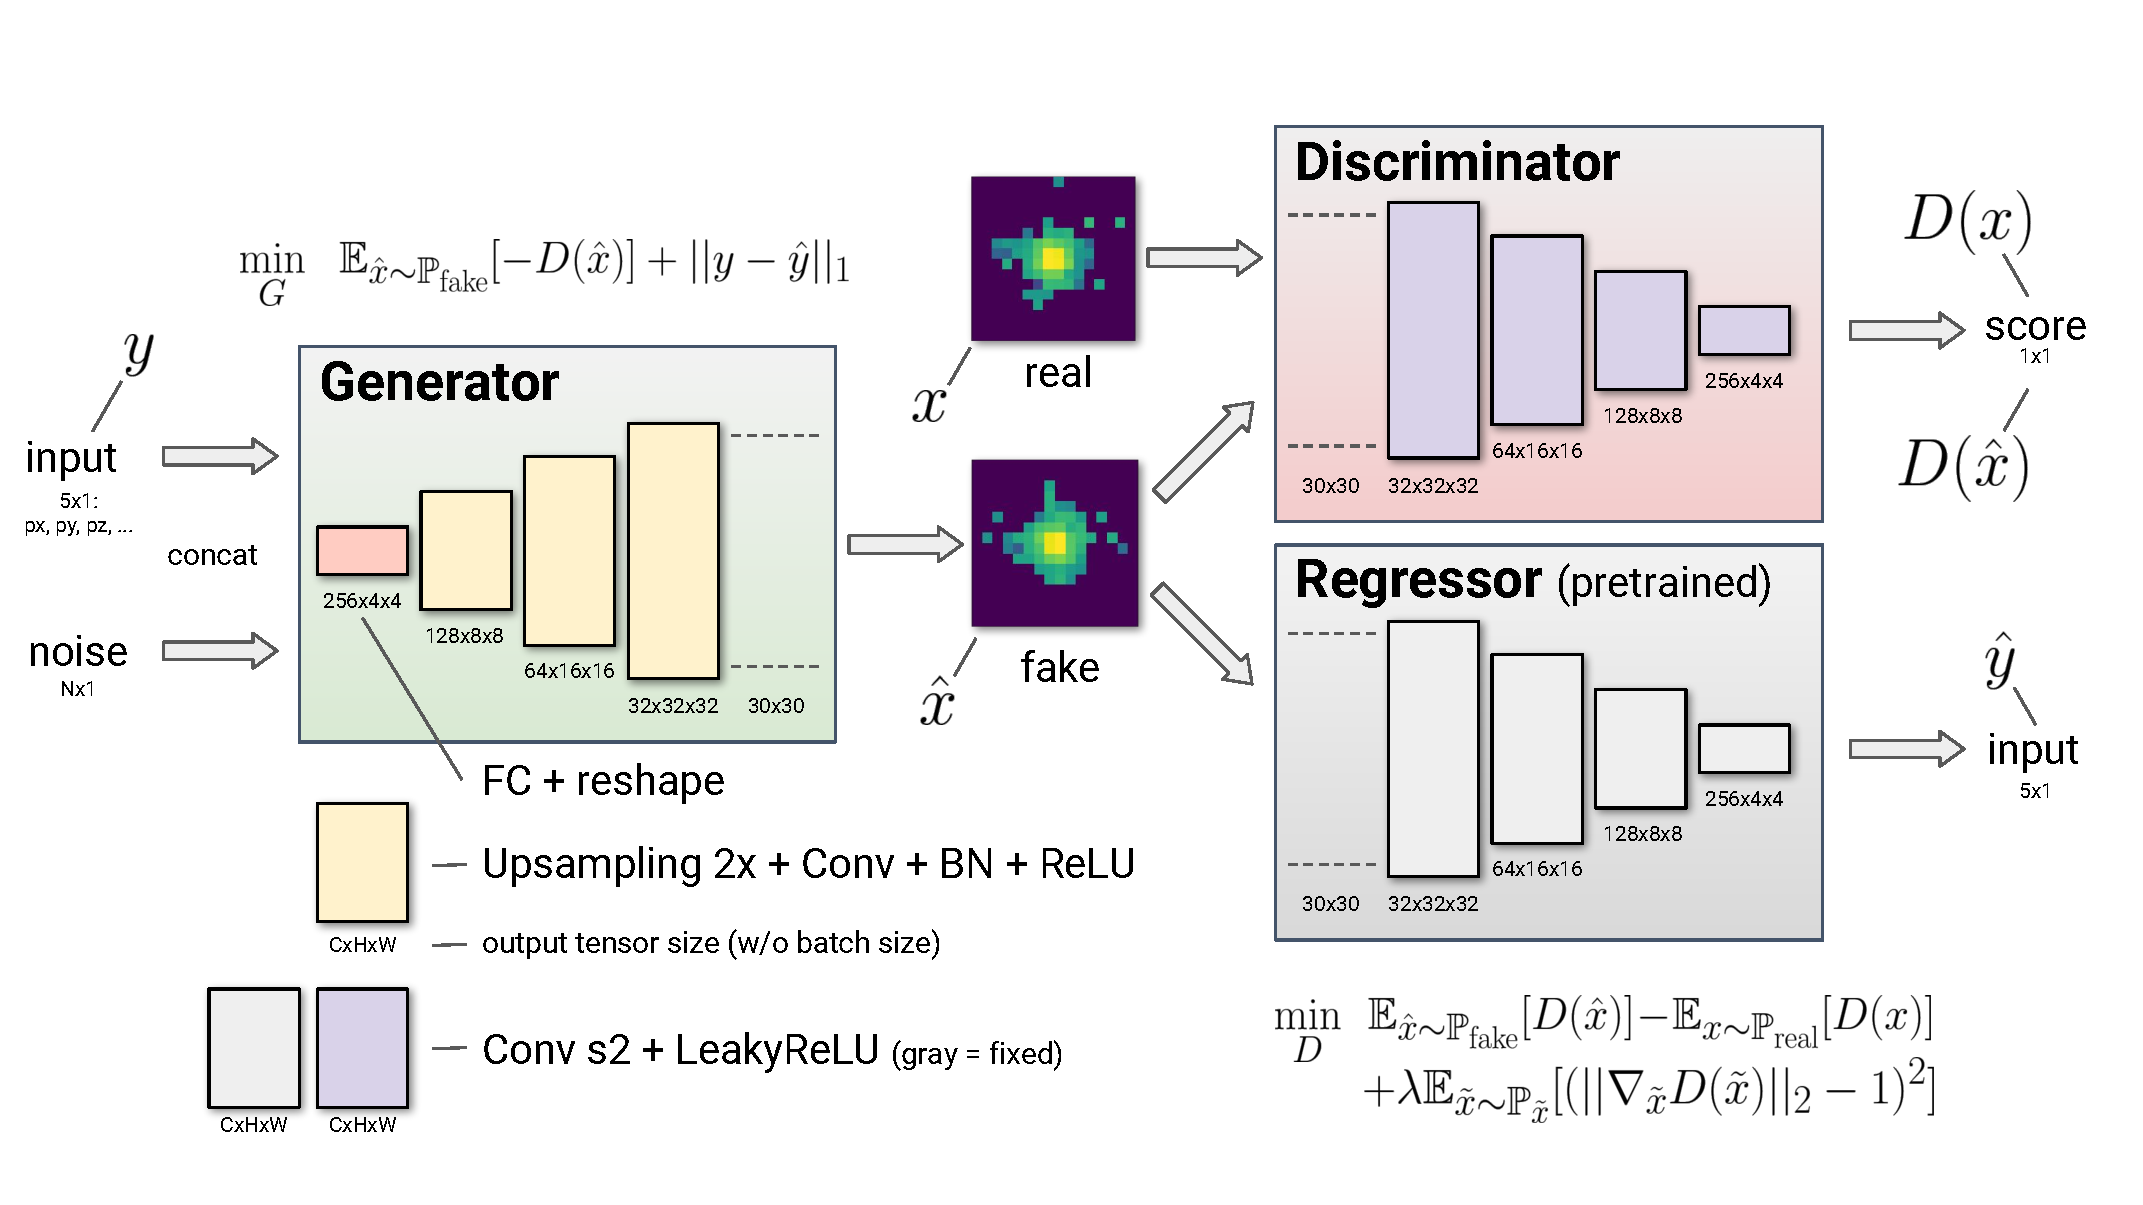
\includegraphics[width=1\textwidth]{figures/model_architecture.pdf}
\caption{Model architecture. Pretrained regressor for the particle parameters prediction makes our model conditional. Thanks to building up the information from the pretrained regressor into the discriminator gradient we learn $G$ to produce a specific calorimeter response.}\label{fig:model}
\end{figure}

How to train WGAN with gradient penalty in conditional manner is described in the following section.

\subsection{Training strategy} \label{sec:training_strategy}
Due to the nature of WGAN loss, conditioning on the continuous value is a non-trivial task. To overcome this issue we suggest to embed a pretrained regressor in our model. We train a neural network to predict the particle parameters by the calorimeter response. As for architecture, it has the same one as the discriminator but with a perceptual loss described in \cite{johnson2016perceptual} because, as we figured out, it works better rather than standard MSE. By building up the information from the pretrained regressor into the discriminator gradient, we obtain the conditional model because we train the generator and the discriminator together. Now the discriminator makes the generator produce a specific calorimeter response.

Matrices from our dataset are pretty sparse because almost all information is located in central cells (see~\cref{fig:real-imgs}). To make optimization process easier we apply a box--cox transformation. This mapping helps to smooth the data that makes the optimization process more stable.
Results obtained with the described model are presented in the following section.
